\documentclass{article}
\usepackage{cite, listings, graphicx, subfigure, amsmath}
\title{EEL6935: Autonomic Computing  Fall 2011\\Homework 2\\Monitoring and
Controlling Xen VMs}
\date{September 29, 2011}
\author{Jorge G\'omez}

\begin{document}
\maketitle
\tableofcontents
\section{Introduction}
  The code used to run all the experiments and make the graphs is listed
  in Appendix~\ref{sec:appendix}. One program ``hw2.py'' runs the
  experiments and dumps the result as a python pickle string---a
  serialized representation of a python dictionary. The other program
  ``hw2\_graph.py'' loads the pickle string and graphs the results of
  the experiments. The following sections will give analysis for each
  section along with a graph of the CPU usage and amount of Free Memory
  in each experiment. The output of the program will also be given as a
  listing at the end of each section.

\section{Experiment \#1}
  In this experiment, no workload was introduced. The virtual machine
  was just monitored in an idle state for five minutes, every 10
  seconds. It was found that using the command xentop in a batch mode
  was sufficient to gather CPU usage (\%) but not the free memory.
  Therefore, vmstat was run on the VM to get the current memory.
  Figure~\ref{fig:ex1} shows the CPU \% very low and constant around 0.1\%.
  The free memory is also constant at around 32 MB. The output of the
  experiment is given in Listing~\ref{lst:ex1}.

  \begin{figure}
    \begin{center}
      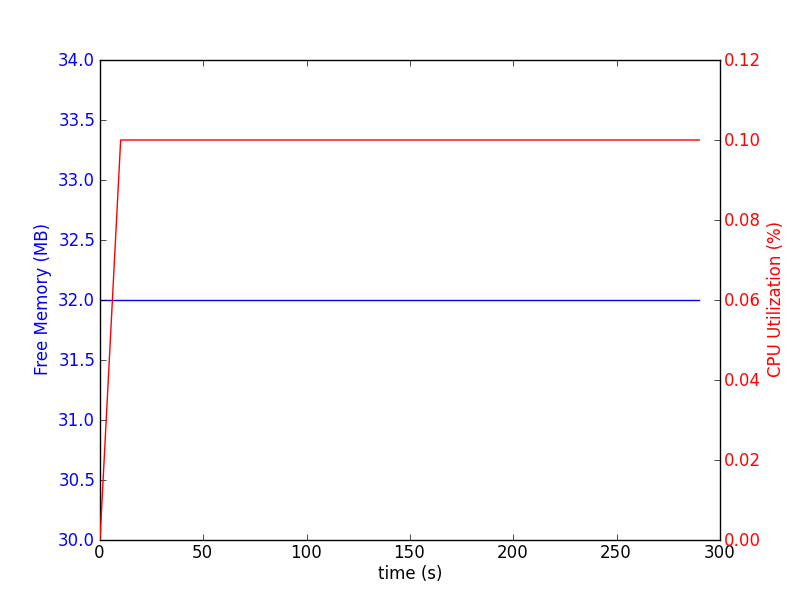
\includegraphics[scale=0.50]{ex1.png} 
      \caption{Results of Experiment \#1 over 5 minutes}
      \label{fig:ex1}
    \end{center}
  \end{figure}

  \lstset{caption={Listing of output of Experiment \#1},label={lst:ex1}}
  \lstinputlisting{ex1.out}

\section{Experiment \#2}
  For the second experiment a workload was introduced. The workload
  performs a matrix multiplication a certain amount of times. In this
  experiment the workload was set to 40. It can be observed that when
  the workload starts, at $t=15$ seconds, the free memory goes down from
  32 MB to 27 MB and the CPU utilization goes up to 100\% from 0\%. The
  Multiplication takes 3 minutes and 12 seconds, as shown in the output,
  and at that time, the memory and CPU utilization go back to there idle
  states.  Figure~\ref{fig:ex2} shows the graph of CPU and memory
  utilization. The output of the experiment is given in
  Listing~\ref{lst:ex2}.

  \begin{figure}
    \begin{center}
      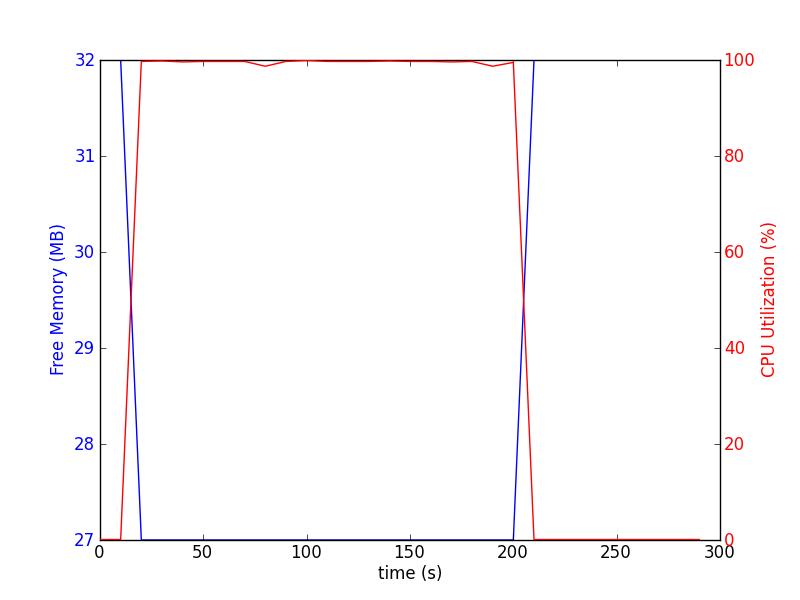
\includegraphics[scale=0.50]{ex2.png} 
      \caption{Results of Experiment \#2 over 5 minutes with workload
      set to 40}
      \label{fig:ex2}
    \end{center}
  \end{figure}

  \lstset{caption={Listing of output of Experiment \#2},label={lst:ex2}}
  \lstinputlisting{ex2.out}

\section{Experiment \#3}
  Experiment \#3 was similar to experiment \#2 except that the workload
  was varied in increments of 10 from 10 to 50. The experiment runs over
  a total of 25 minutes, as shown in Figure~\ref{fig:ex3}. As the
  workload increases, one can see that the amount of time the VM is
  active increases.  The output of the experiment is given in
  Listing~\ref{lst:ex3}.

  \begin{figure}
    \begin{center}
      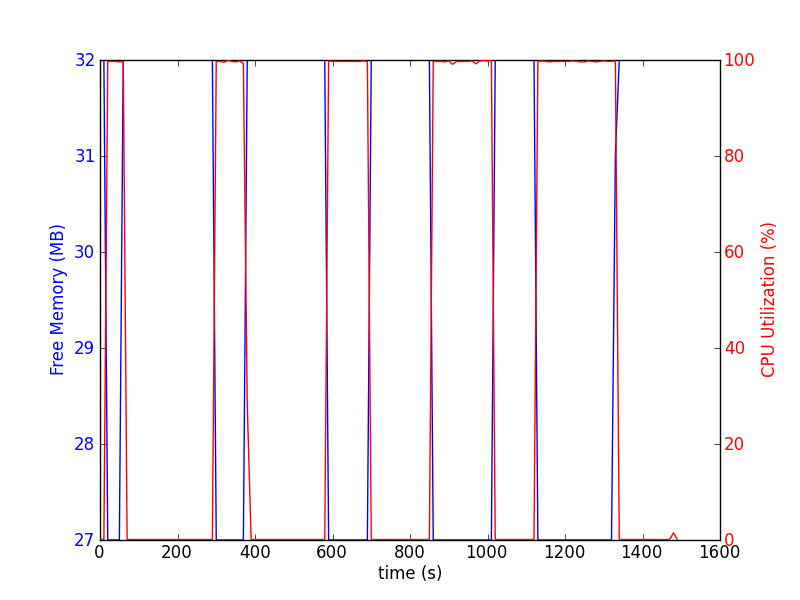
\includegraphics[scale=0.50]{ex3.png} 
      \caption{Results of Experiment \#3 over 25 minutes with workload
      varied from 10 to 50 in increments of 10}
      \label{fig:ex3}
    \end{center}
  \end{figure}

  \lstset{caption={Listing of output of Experiment \#3},label={lst:ex3}}
  \lstinputlisting{ex3.out}

\section{Experiment \#4}
  For the final experiment, the procedure of experiment \#3 was repeated
  with different settings of the VM. The CPU cap was set to 50\% and
  75\% and the memory allocated to the VM was set to 128 and 256 MB. The
  cases of 100\% CPU cap and 512 MB of allocated memory were not
  considered because they are identical to the previous experiment.
  Figures~\ref{fig:ex4CPU50}, \ref{fig:ex4CPU75}, \ref{fig:ex4Mem128}, and
  \ref{fig:ex4Mem256}
  show the results of the experiment \#3 procedure for each of these
  cases. As the figures show, limiting the CPU cycles allocated to the
  VM have the effect of making the work take longer. The memory
  allocation had no effect though, probably due to the small size of the
  matrix being computed. The output of the experiment is given in
  Listing~\ref{lst:ex4}.

  \begin{figure}
    \begin{center}
      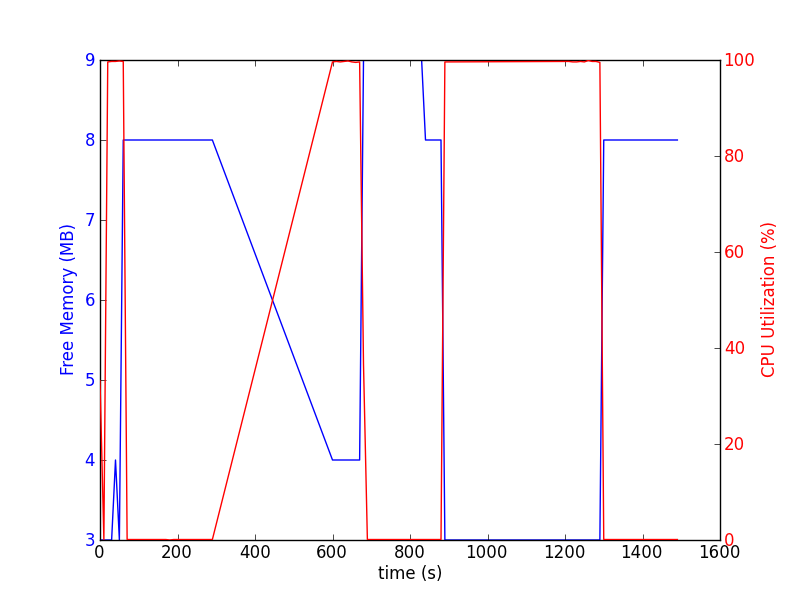
\includegraphics[scale=0.50]{ex4Mem=128.png} 
      \caption{Results of Experiment \#3 (only workload of 10, 20, and
      30) with only 128 MB of memory allocated to the VM}
      \label{fig:ex4Mem128}
    \end{center}
  \end{figure}

  \begin{figure}
    \begin{center}
      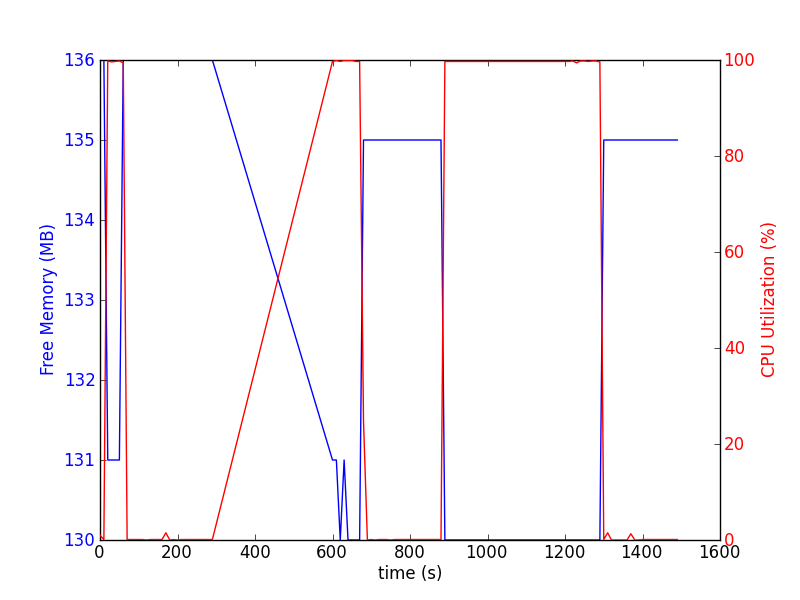
\includegraphics[scale=0.50]{ex4Mem=256.png} 
      \caption{Results of Experiment \#3 (only workload of 10, 20, and
      30) with only 256 MB of memory allocated to the VM}
      \label{fig:ex4Mem256}
    \end{center}
  \end{figure}

  \begin{figure}
    \begin{center}
      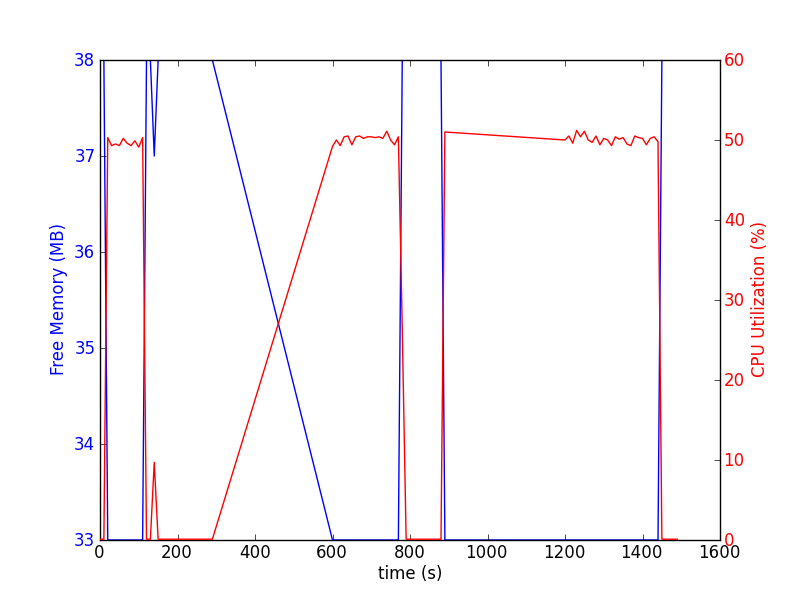
\includegraphics[scale=0.50]{ex4Cap=50.png} 
      \caption{Results of Experiment \#3 (only workload of 10, 20, and
      30) with only 50\% CPU time allocated to the VM}
      \label{fig:ex4CPU50}
    \end{center}
  \end{figure}

  \begin{figure}
    \begin{center}
      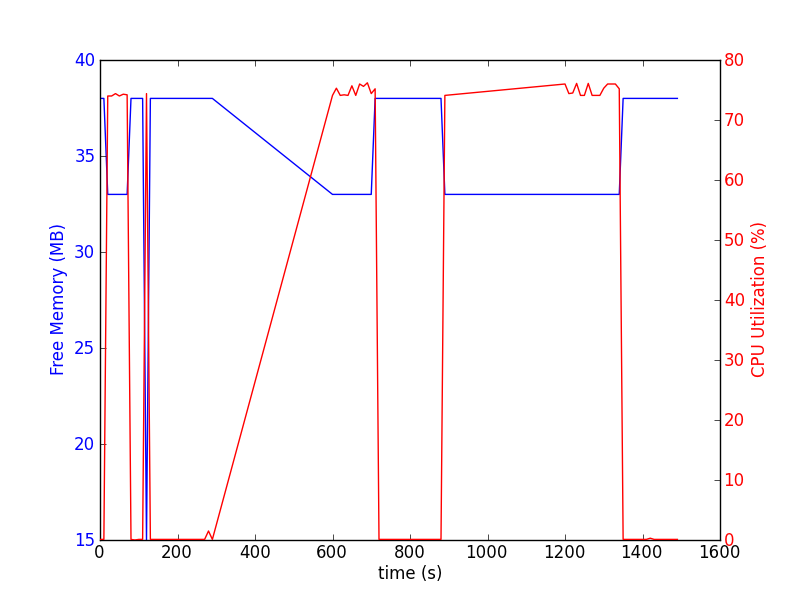
\includegraphics[scale=0.50]{ex4Cap=75.png} 
      \caption{Results of Experiment \#3 (only workload of 10, 20, and
      30) with only 75\% CPU time allocated to the VM}
      \label{fig:ex4CPU75}
    \end{center}
  \end{figure}

  \lstset{caption={Listing of output of one run in Experiment \#4},label={lst:ex4}}
  \lstinputlisting{ex4.out}

\section{Conclusions}
  This homework assignment helped greatly in learning how to monitor and
  control Xen VM systems---a lesson which I will definitely use in my
  professional life. Unfortunately, the last experiment didn't run
  perfectly and took a lot longer to complete than expected, but, with a
  few tweaks, the code written here should serve as a great base for
  future experiments. I look forward to doing more assignments in this
  topic.

\appendix
\section{Code Listings}
\label{sec:appendix}
  \lstset{language=Python,caption={Python program used to gather
  data},label={lst:hw2}}
  \lstinputlisting{../hw2.py}

  \lstset{language=Python,caption={Python program used to make the
  charts},label={lst:hw2graph}}
  \lstinputlisting{../hw2_graph.py}

\end{document}
